\documentclass[10pt]{beamer}

\usepackage{fontspec}

%% Minted setup (syntax highlighting)
\usepackage[outputdir=latex.out]{minted}
\usemintedstyle{vs}
\setminted{fontsize=\footnotesize}
\newminted[code]{scala}{gobble=0, escapeinside=@@}
\newenvironment{slide}[2][]
  {\begin{frame}[fragile,environment=slide,#1]{#2}}
  {\end{frame}}
\newcommand\makemintedshortinline[2]{%
  \catcode`#2=13
  \begingroup%
  \lccode`\~=`#2
  \lowercase{\endgroup\protected\def~{\mintinline[escapeinside=@@]{#1}~}}%
}
\renewcommand{\fcolorbox}[4][]{#4}

%% Beamer theme setup
\usetheme[block=fill]{metropolis}
\setbeamercolor{progress bar}{bg=black, fg=black}
\setbeamercolor{title separator}{bg=black, fg=black}
\setbeamercolor{progress bar in head/foot}{bg=black, fg=black}
\setbeamercolor{progress bar in section page}{bg=black, fg=black}
\setbeamercovered{transparent}

\usepackage[sorting=none, backend=biber, maxbibnames=9]{biblatex}
% \settowidth\labelnumberwidth{\usebeamertemplate*{bibliography item}}
\AtEveryBibitem{\clearfield{note}}
\AtEveryBibitem{\clearfield{volume}}
\AtBeginBibliography{\small}
\bibliography{bibliography}

\usepackage{textpos}
\usepackage{ulem}
\usepackage{xspace}
\usepackage{mathtools}
\usepackage{booktabs}
\usepackage{ulem}

\usepackage[autostyle=false, style=english]{csquotes}
\MakeOuterQuote{"}

\usepackage{xcolor}
\definecolor{typeColor}{HTML}{2B91B0}
\definecolor{implColor}{HTML}{57B5E8}
\definecolor{singColor}{HTML}{009E73}
\definecolor{mtpeColor}{HTML}{9400D4}
\definecolor{FAFAFA}{HTML}{FAFAFA}
\newcommand{\tp}[1]{\color{typeColor}#1}

\usepackage{tikz}
\usetikzlibrary{decorations.pathreplacing,positioning, arrows.meta}

\def\checkmark{\textcolor{green}{\tikz\fill[scale=0.6](0,.35) -- (.25,0) -- (1,.7) -- (.25,.15) -- cycle;}}
\def\cross{$\mathbin{\tikz [x=1.4ex,y=1.4ex,line width=.2ex, red] \draw (0,0) -- (1,1) (0,1) -- (1,0);}$}

\title{Abstractions for Type-Level Programming}
\date{Wednesday, 25 May 2022}
\author{Olivier Blanvillain}

\makemintedshortinline{scala}\|

\newcommand{\timeline}[5] {
  \begin{tikzpicture}
    \draw[lightgray!#5!black, thick, -Triangle] (0,0) -- (10cm,0);
    \foreach \x in {0,1,...,6}
    \draw[lightgray!#5!black] (\x*1.4 cm,3pt) -- (\x*1.4 cm,-3pt);

    \foreach \x/\descr in {0/2016,1/2017,2/2018,3/2019,4/2020,5/2021,6/2022}
    \node[lightgray!#5!black, font=\scriptsize, text height=1.75ex,
    text depth=.5ex] at (\x*1.4,-.3) {$\descr$};

    \fill[lightgray!#1!implColor] (0.25, 0.5) circle (4pt) node[lightgray!#1!black,align=center,above=7pt,font=\small]{DataFrame\\Library};

    \draw[lightgray!#2!singColor, line width=4pt]
    (2.25*1.4,.5) -- (4.417*1.4,.5) node[lightgray!#2!black,midway,above=5pt,font=\small]{Generalized Singletons};

    \draw[lightgray!#3!mtpeColor, line width=4pt]
    (2.5*1.4,-.7) -- (6.15*1.4,-.7) node[lightgray!#3!black,midway,below=5pt,font=\small]{Match Types};
    \draw[thick,lightgray!#3!mtpeColor,-Triangle,line width=1.2pt] (6.15*1.4,-.7) -- (6.25*1.4,-.7);

    \fill[lightgray!#4!mtpeColor] (6.1*1.4, 0.5) circle (4pt) node[lightgray!#4!black,align=center,above=7pt,font=\small]{Regex\\Library};
  \end{tikzpicture}
}

\begin{document}

\maketitle

\begin{slide}{Welcome!}
\Large
\begin{center}
Bienvenue à ma déf\textcolor{typeColor}{ense} de thèse !\\
\phantom{Bienvenue à ma} déf\textcolor{implColor}{anse} \phantom{de thèse !}\\
\phantom{Bienvenue à ma} déf\textcolor{singColor}{ence} \phantom{de thèse !}\\
\phantom{Bienvenue à ma} déf\textcolor{mtpeColor}{ance} \phantom{de thèse !}\\
\end{center}
\end{slide}

\begin{slide}{Welcome!}
\Large
\begin{center}
Bienvenue à ma souten\textcolor{typeColor}{ense} de thèse !\\
\phantom{Bienvenue à ma} souten\textcolor{implColor}{anse} \phantom{de thèse !}\\
\phantom{Bienvenue à ma} souten\textcolor{singColor}{ence} \phantom{de thèse !}\\
\phantom{Bienvenue à ma} souten\textcolor{mtpeColor}{ance} \phantom{de thèse !}\\
\end{center}
\end{slide}

\begin{slide}{Spell checkers to the rescue}
\begin{center}
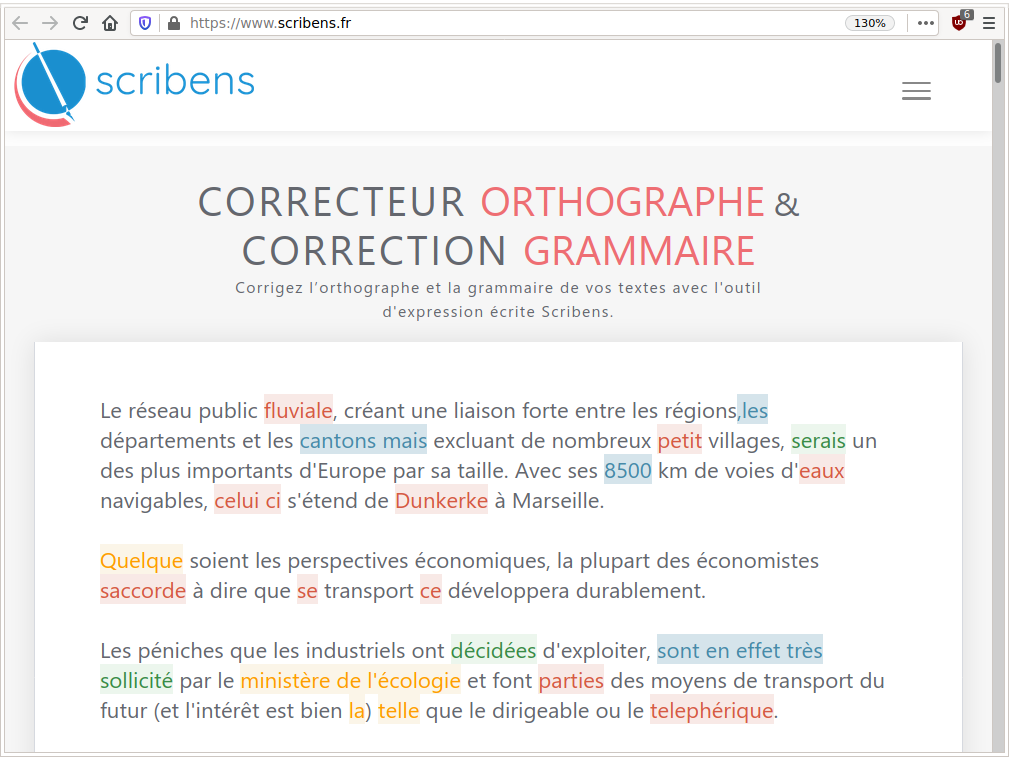
\includegraphics[width=\textwidth]{figures/scribens.png}
\end{center}
\end{slide}

\section{Programming Methods Laboratory\hspace{-2pt}}

\begin{slide}{An analogy...}
\begin{center}
\Large
Programming $\longleftrightarrow$ Poetry
\vspace{10pt}


\includegraphics[width=0.5\textwidth]{figures/poetry.jpg}
\end{center}
\end{slide}

\begin{slide}{An analogy...}
\begin{center}
\Large
Scala $\longleftrightarrow$ La Langue Française
\vspace{10pt}

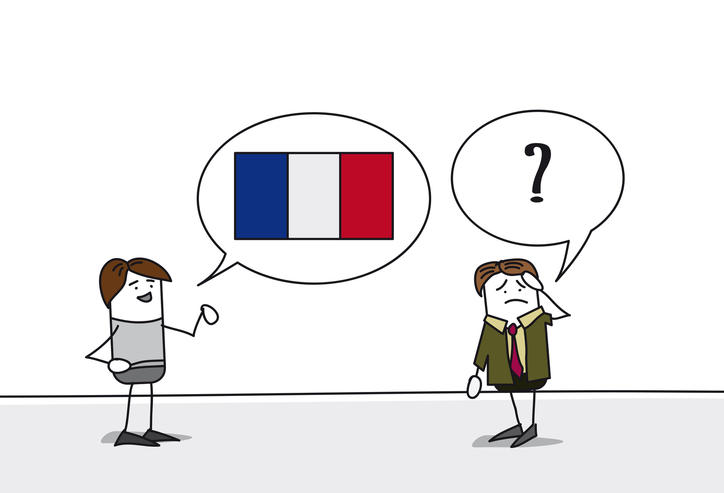
\includegraphics[width=0.6\textwidth]{figures/fr.jpg}
\end{center}
\end{slide}

\begin{slide}{An analogy...}
\begin{center}
\Large
Compiler $\longleftrightarrow$ Spell checker
\vspace{10pt}

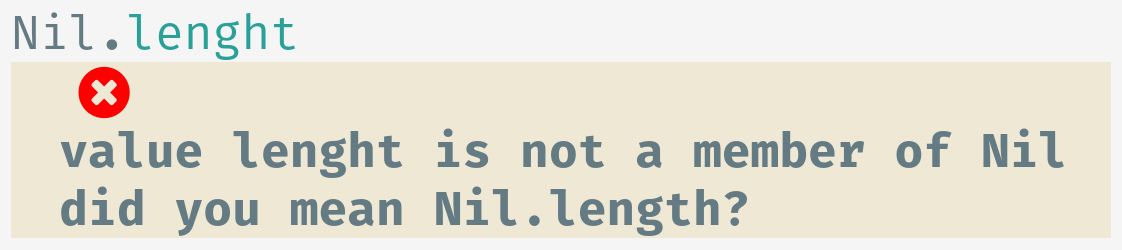
\includegraphics[width=\textwidth]{figures/nil.png}
\end{center}
\end{slide}

\begin{slide}{An analogy...}
\begin{center}
\begin{minipage}{0.45\textwidth}
\Large
Standard library $\longleftrightarrow$
\end{minipage}
\begin{minipage}{0.45\textwidth}
\vspace{10pt}
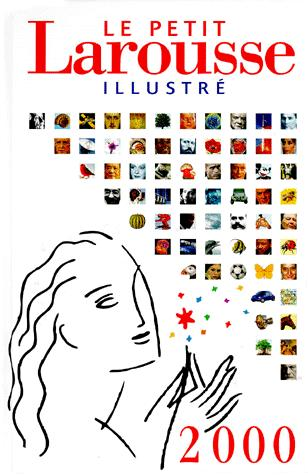
\includegraphics[width=\textwidth]{figures/larousse.jpg}
\end{minipage}
\end{center}
\end{slide}

\begin{slide}{An analogy...}
\begin{center}
\begin{minipage}{0.37\textwidth}
\Large
Type system $\longleftrightarrow$
\end{minipage}
\begin{minipage}{0.45\textwidth}
\vspace{10pt}
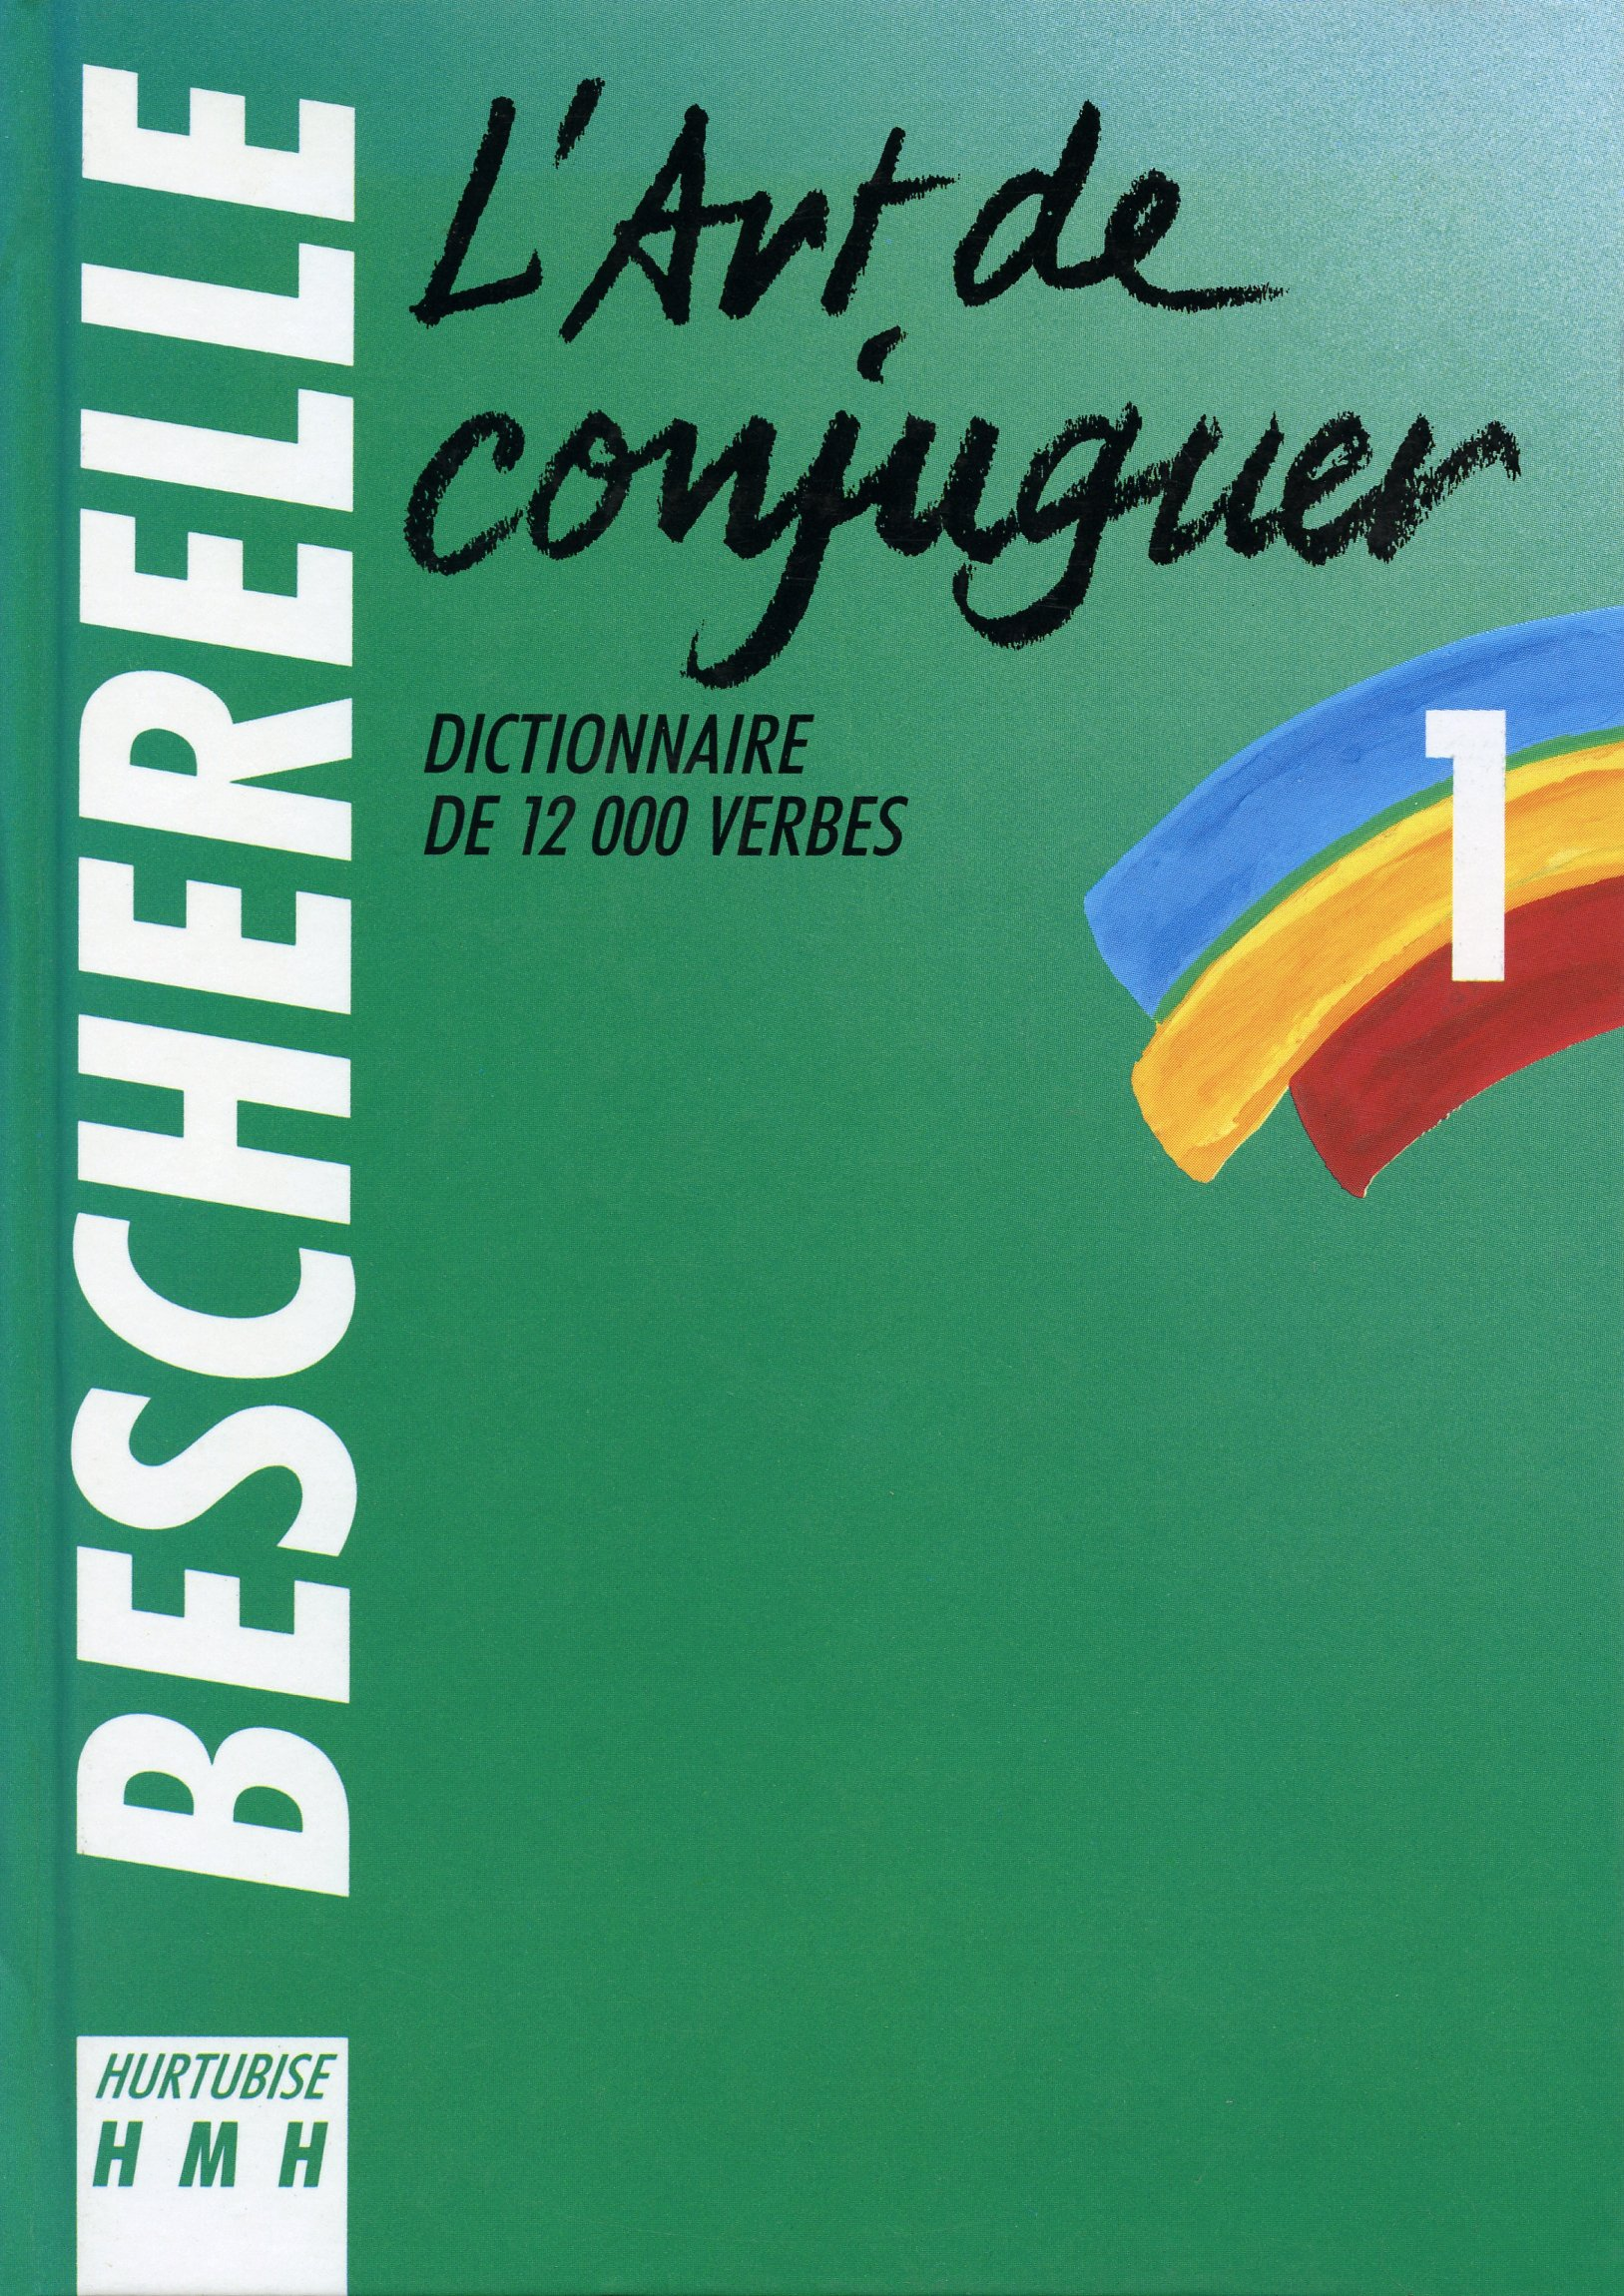
\includegraphics[width=\textwidth]{figures/bescherelle.jpg}
\end{minipage}
\end{center}
\end{slide}

\begin{slide}{LAMP -- Poetry Methods Laboratory}
\large
\begin{itemize}
  \item Scala $\longleftrightarrow$ La Langue Française
  \item Compiler $\longleftrightarrow$ Spell checker
  \item Standard library $\longleftrightarrow$ Le Petit Larousse Illustré
  \item Type system $\longleftrightarrow$ Bescherelle (rêgles de grammaires)
\end{itemize}
\end{slide}

\section{My Contribution}

\begin{slide}{My contribution}
\Large
My contribution:

A new Scala feature for type-level programming.

I will give you an intuition using examples:

\begin{itemize}
  \item A poetry example
  \item A math example
  \item A programming example
\end{itemize}
\end{slide}

\begin{slide}{Type-level programming: poetry example}
\Large
What do I mean by Type-Level Programming?

A way to \emph{customize} the spell checker.

\begin{center}
\hspace{20pt}
\begin{minipage}{0.45\textwidth}%
\phantom{-- en alexandrin}\\
\phantom{Roses are red,}\\
\phantom{violets are blue,}\\
\phantom{so are you.}
\end{minipage}
\end{center}
\end{slide}

\begin{slide}{Type-level programming: poetry example}
\Large
What do I mean by Type-Level Programming?

A way to \emph{customize} the spell checker.

\begin{center}
\hspace{20pt}
\begin{minipage}{0.45\textwidth}%
\phantom{-- en alexandrin}\\
Roses are red,\\
violets are blue,\\
so are you.
\end{minipage}
\end{center}
\end{slide}

\begin{slide}{Type-level programming: poetry example}
\Large
What do I mean by Type-Level Programming?

A way to \emph{customize} the spell checker.

\begin{center}
\hspace{20pt}
\begin{minipage}{0.45\textwidth}%
\textcolor{blue}{"En alexandrin"}\\
Roses are red,\\
violets are blue,\\
so are you. \textcolor{red}{\cross}
\end{minipage}
\end{center}
\end{slide}


\begin{slide}{Type-level programming: poetry example}
\Large
What do I mean by Type-Level Programming?

A way to \emph{customize} the spell checker.

\begin{center}
\hspace{20pt}
\begin{minipage}{0.45\textwidth}%
\textcolor{blue}{"En alexandrin"}\\
Roses are red,\\
violets are blue,\\
and so are you. \checkmark
\end{minipage}
\end{center}
\end{slide}

\begin{slide}{Type-level programming: math example}
\Large
How many ways are there to pick 13 cards from a 52-card deck?
\begin{center}
\begin{minipage}{0.6\textwidth}
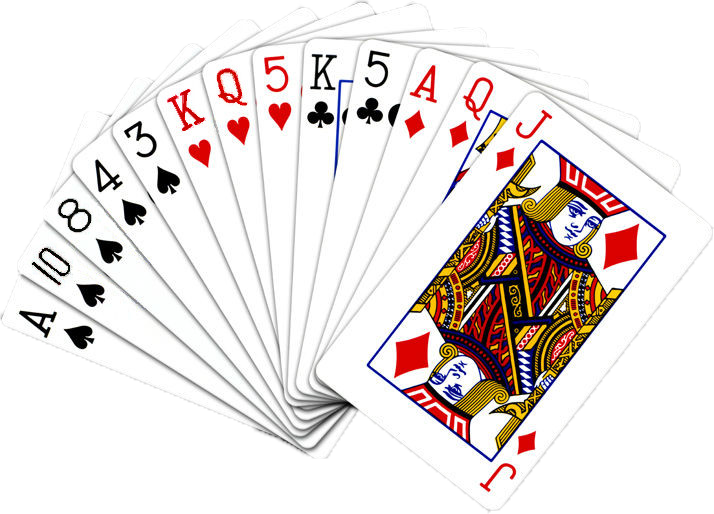
\includegraphics[width=\textwidth]{figures/cards.png}
\end{minipage}
\begin{minipage}{0.2\textwidth}
$$
\phantom{binom{52}{13}}
$$
\end{minipage}
\end{center}
\end{slide}

\begin{slide}{Type-level programming: math example}
\Large
How many ways are there to pick 13 cards from a 52-card deck?
\begin{center}
\begin{minipage}{0.6\textwidth}
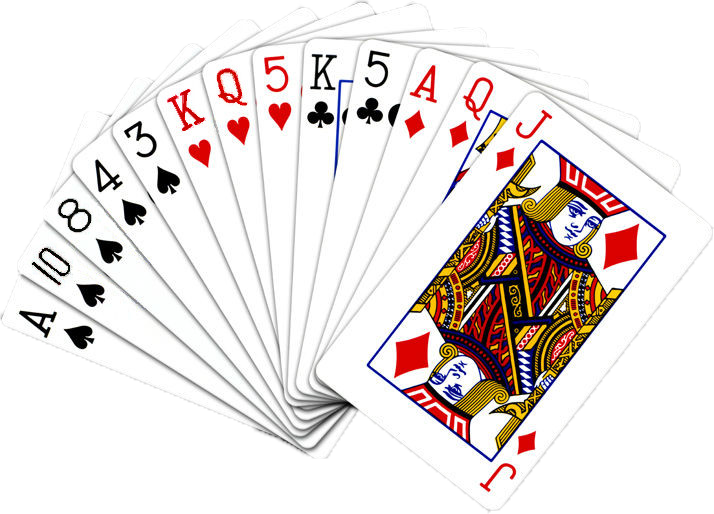
\includegraphics[width=\textwidth]{figures/cards.png}
\end{minipage}
\begin{minipage}{0.2\textwidth}
$$
\binom{52}{13}
$$
\end{minipage}
\end{center}
\end{slide}

\begin{slide}{Type-level programming: math example}
\Large
The binomial coefficients are defined as follows:

$$
\binom{\textcolor{typeColor}{n}}{\textcolor{mtpeColor}{k}} = \frac{\textcolor{typeColor}{n}!}{\textcolor{mtpeColor}{k}!(\textcolor{typeColor}{n} - \textcolor{mtpeColor}{k})!}
$$
\end{slide}

\begin{slide}{Type-level programming: math example}
\Large
The $\binom{\textcolor{typeColor}{n}}{\textcolor{mtpeColor}{k}}$ symbol usually read as:

\begin{itemize}
  \item "\textcolor{typeColor}{n} choose \textcolor{mtpeColor}{k}" in English
  \item "\textcolor{mtpeColor}{k} parmis \textcolor{typeColor}{n}" in French
\end{itemize}
\pause

Programmers might confuse \textcolor{typeColor}{n} \& \textcolor{mtpeColor}{k}? Should it be

\begin{itemize}
\item binomialCoefficient(\textcolor{typeColor}{n}, \textcolor{mtpeColor}{k}) or
\item binomialCoefficient(\textcolor{mtpeColor}{k}, \textcolor{typeColor}{n})?
\end{itemize}
\end{slide}

\begin{slide}{Type-level programming: math example}
\Large
\textbf{def} binomialCoefficient(\textcolor{typeColor}{n}: Int, \textcolor{mtpeColor}{k}: Int): Int\\
\phantom{def }

binomialCoefficient(52, 13) \checkmark

binomialCoefficient(13, 52) \checkmark
\end{slide}

\begin{slide}{Type-level programming: math example}
\Large
\textbf{def} binomialCoefficient(\textcolor{typeColor}{n}: Int, \textcolor{mtpeColor}{k}: Int)\\
\phantom{def }(\textbf{implicit} ev: \textcolor{typeColor}{n}.type >= \textcolor{mtpeColor}{k}.type \raisebox{-.06\baselineskip}{=}:\raisebox{-.06\baselineskip}{=} true): Int

binomialCoefficient(52, 13) \checkmark

binomialCoefficient(13, 52) \cross
\end{slide}

\begin{slide}{Type-level programming: regular expression example}
\Large
A regular expression is a simple tool to validate and extract data from text.
\vspace{10pt}

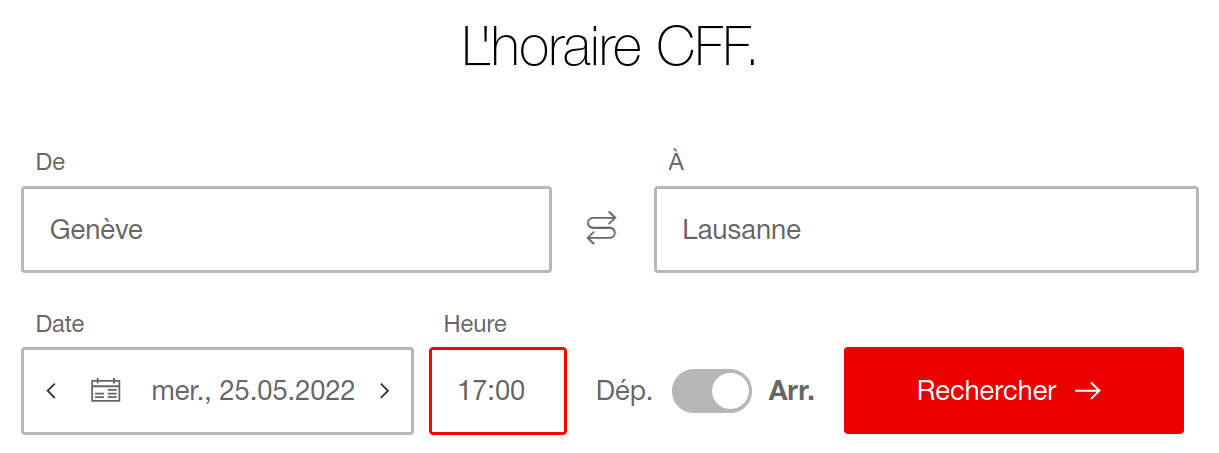
\includegraphics[width=\textwidth]{figures/cff.png}
\end{slide}

\begin{slide}{Type-level programming: regular expression example}
\begin{center}
\renewcommand{\arraystretch}{1.2}
\begin{tabular}{@{}llrrr@{}}
\toprule
|input| & |pattern| & |out[0]| & |out[1]| & |out[2]| \\
\midrule
|"17:00"| & |"(\d+)[.:h](\d+)"| & |"17"| & |"00"|  & \\
\pause
|"25.05.2022"| & |"(\d+).(\d+).(\d+)"| & |"25"| & |"05"| & |"2022"| \\
\bottomrule
\end{tabular}
\end{center}
\end{slide}

\begin{slide}{Type-level programming: regular expression example}
\begin{center}
\renewcommand{\arraystretch}{1.2}
\begin{tabular}{@{}llrrr@{}}
\toprule
|input| & |pattern| & |out[0]| & |out[1]| & |out[2]| \\
\midrule
|"17:00"| & |"(\d+)[.:h](\d+)"| & |"17"| & |"00"|  & \cross \\
|"25.05.2022"| & |"(\d+).(\d+).(\d+)"| & |"25"| & |"05"| & |"2022"| \\
\bottomrule
\end{tabular}
\end{center}
\end{slide}

\begin{slide}{Timeline of my PhD}
\timeline{0}{0}{0}{0}{0}
\end{slide}

\begin{slide}{Conclusion}
\Large
In this talk, I presented an analogy to explain what we do in the \sout{Programming} Poetry Methods Laboratory.

I also presented a few example to illustate my contribution:

\begin{center}
  
\includegraphics[width=0.25\textwidth]{figures/poetry.jpg}
  \hspace{10pt}
  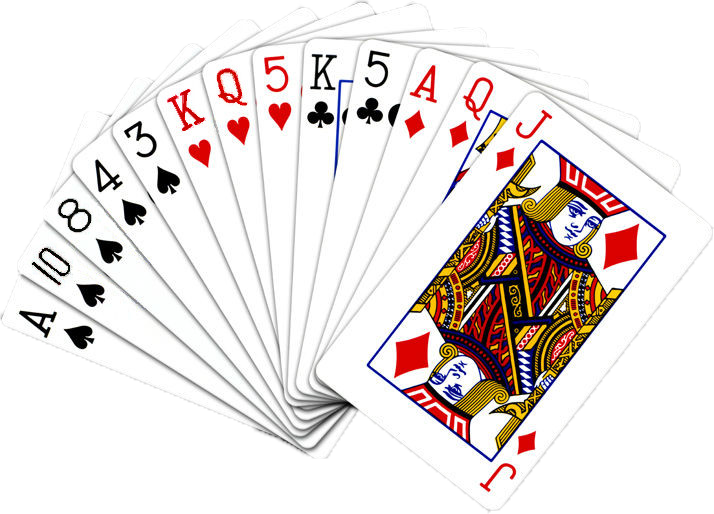
\includegraphics[width=0.32\textwidth]{figures/cards.png}
  \hspace{10pt}
  
\includegraphics[width=0.25\textwidth]{figures/cff-logo.jpg}
\end{center}

\end{slide}

\begin{slide}{Thank you!}
\begin{center}
\Huge Thank you!
\end{center}
\end{slide}

\end{document}
